% Fig. 4.11 / CH4_FIGURE_SPECS.md -- the identity t_{alpha/2}(nu) =
%   sqrt(F_alpha(1, nu)) drawn as two panels joined by an arrow: the two
%   symmetric tails of t(nu), once squared, land on the one right tail of
%   F(1, nu).
% Source: mathstatch4.tex lines 4708-4790, a tabular whose first and third
%   cells hold a tikzpicture each and whose middle cell holds
%   $\xRightarrow[]{~F=T^2~}$.  CH4_FIGURE_SPECS 3.2 requires the arrow to be
%   drawn into the web figure, since it is what ties the two panels together.
%
%   Left panel (manuscript lines 4710-4751): t density drawn with nu = 10 but
%   marked nu, domain -3:3 at samples=400, xmin=-3.2, xmax=3.2, ymin=0,
%   ymax=0.41, bottom axis line only (axis y line=none), no y tick labels, no
%   axis names.  Three x ticks at -2.228139, 0 and 2.228139 marked
%   $-t_{\alpha/2}(\nu)$, $0$ and $t_{\alpha/2}(\nu)$; gray tails at opacity
%   0.2 on [-3, -2.228139] and [2.228139, 3]; a segment dropped to the axis
%   from each of the two points, both at height 0.04238497; legend $t(\nu)$.
%
%   Right panel (manuscript lines 4754-4785): F density drawn with (1, 10)
%   but marked (1, nu), domain 0:6 at samples=600, xmin=0, xmax=6.2, ymin=0,
%   ymax=0.5, bottom axis line plus a y axis at x = 0 (axis y line=middle),
%   no y tick labels, no axis names.  Two x ticks at 0 and 4.964603 marked
%   $0$ and $\mathcal{F}_{\alpha}(1, \nu)$; a gray tail at opacity 0.2 on
%   [4.964603, 6]; a segment dropped to the axis at 4.964603 from height
%   0.01902259; legend $\mathcal{F}(1, \nu)$.
%
% The two densities, written out so that no gamma function is evaluated at
% run time; the two constants are the same number because F = T^2:
%   t(10):    f(x) = 0.38910838 (1 + x^2/10)^{-11/2}
%   F(1,10):  f(x) = 0.38910838 x^{-1/2} (1 + x/10)^{-11/2}
% with 0.38910838 = Gamma(11/2)/(sqrt(10 pi) Gamma(5)).  These reproduce the
% four heights the manuscript hard-codes: f_{t(10)}(2.228139) = 0.04238497
% and f_{F(1,10)}(4.964603) = 0.01902259, and 2.228139^2 = 4.964603, which is
% the identity the figure is about.
%
% Departures from the manuscript figure, all required by the site specs:
%
% 1. Colour and line width per CH3_FIGURE_SPECS 1: curves and axes in
%    journalink at 0.8pt, tails in journalaccent at fill opacity 0.15 rather
%    than gray at 0.2.
%
% 2. The manuscript's legend entry becomes a label written at the curve
%    itself, per CH2 spec 1.9, which prefers that to a legend box; with one
%    curve to a panel there is nothing for a legend to tell apart.  Each label
%    sits in the upper corner the density leaves empty.
%
% 3. The tick label $0$ is set on a second row in both panels.  On one row the
%    box of $t_{\alpha/2}(\nu)$ would stand 0.53cm clear of the box of $0$,
%    under the 0.6cm of CH2 spec 1.3; on two rows the two tail-point labels,
%    which are what the figure is about, clear each other by 1.01cm.
%
% 4. The F density runs to infinity as x approaches 0, and pgfplots cuts it at
%    ymax; the same cut is made here by starting the curve at x = 0.3953,
%    which is where the density equals 0.5.
%
% 5. The manuscript's two panels are the same width but carry different
%    density ranges (0.41 against 0.5).  Their plot boxes are given the same
%    height here, 2.60cm, so that the arrow runs level between them.
%
% Size and type.  Drawing range 7.41cm wide, inside the 9.0cm cap of CH2 spec
% 1.3.  A mark of S pt shows at S x 0.99626 x <display width> / <native width>
% px.  The figure sits inside a topic-proof, which indents the body column by
% 1.1em plus a 2px rule, so a topic-figure--wide there is about 328px on a
% 390px phone.  The smallest mark is the alpha and the 2 of the fraction in
% $t_{\alpha/2}(\nu)$, at scriptscript size, which
% \DeclareMathSizes{10}{10}{9}{8} holds at 8pt rather than the 5pt of the
% default math sizes.
\documentclass[tikz,border=2pt]{standalone}
\usepackage{amsmath}
\usepackage{amssymb}
\usepackage{xcolor}
\usetikzlibrary{arrows.meta}
\DeclareMathSizes{10}{10}{9}{8}

\definecolor{journalink}{HTML}{1F1C18}
\definecolor{journalmuted}{HTML}{8A7F72}
\definecolor{journalaccent}{HTML}{9C2D2D}

\newcommand{\tten}[1]{0.38910838*pow(1+(#1)*(#1)/10,-5.5)}
\newcommand{\fone}[1]{0.38910838*pow((#1),-0.5)*pow(1+(#1)/10,-5.5)}

\begin{document}
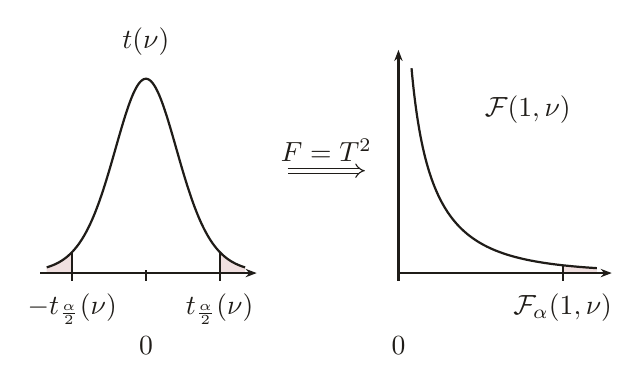
\begin{tikzpicture}[
  x=1cm,
  y=1cm,
  every node/.style={font=\normalsize, journalink},
  axis/.style={journalink, line width=0.8pt, -{Stealth[length=4pt]}},
  tick/.style={journalink, line width=0.8pt},
  curve/.style={journalink, line width=0.8pt},
  drop/.style={journalink, line width=0.8pt},
  tail/.style={journalaccent, fill opacity=0.15}
]
  % ================= left panel: the t density ==========================
  \begin{scope}[xshift=0cm, x=0.42cm, y=6.34cm]
    \fill[tail] (-3,0) -- (-2.228139,0) -- (-2.228139,0.04238497)
      -- plot[domain=-2.228139:-3, samples=120, smooth] (\x,{\tten{\x}})
      -- cycle;
    \fill[tail] (2.228139,0) -- (3,0) -- (3,0.01141862)
      -- plot[domain=3:2.228139, samples=120, smooth] (\x,{\tten{\x}})
      -- cycle;

    \draw[curve] plot[domain=-3:3, samples=260, smooth] (\x,{\tten{\x}});

    \draw[axis] (-3.2,0) -- (3.35,0);

    \draw[drop] (-2.228139,0.04238497) -- (-2.228139,0);
    \draw[drop] (2.228139,0.04238497) -- (2.228139,0);

    \foreach \p in {-2.228139, 0, 2.228139}
      \draw[tick] ([yshift=0.035cm]\p,0) -- ([yshift=-0.106cm]\p,0);

    \node[anchor=north, inner sep=0pt] at ([yshift=-0.25cm]-2.228139,0)
      {$-t_{\frac{\alpha}{2}}(\nu)$};
    \node[anchor=north, inner sep=0pt] at ([yshift=-0.25cm]2.228139,0)
      {$t_{\frac{\alpha}{2}}(\nu)$};
    \node[anchor=north, inner sep=0pt] at ([yshift=-0.80cm]0,0) {$0$};

    % Curve label above the peak, placed as in tail-identity-z-to-chisq.tex so
    % that the two figures match; set 0.435 high it clears the peak, 0.3891,
    % by 0.29cm.
    \node[anchor=south, inner sep=0pt] at (0,0.435) {$t(\nu)$};
  \end{scope}

  % ================= the arrow ==========================================
  \draw[journalink, line width=0.4pt, double, double distance=1.4pt,
        -{Implies[length=5pt]}] (1.80,1.30) -- (2.78,1.30);
  \node[anchor=south, inner sep=2pt] at (2.29,1.34) {$F=T^{2}$};

  % ================= right panel: the F density =========================
  \begin{scope}[xshift=3.207cm, x=0.42cm, y=5.20cm]
    \fill[tail] (4.964603,0) -- (6,0) -- (6,0.01198100)
      -- plot[domain=6:4.964603, samples=120, smooth] (\x,{\fone{\x}})
      -- cycle;

    % The density passes 0.5, the manuscript's ymax, at x = 0.3953; pgfplots
    % cuts it there and so does this.
    \draw[curve] plot[domain=0.3953:6, samples=320, smooth]
      (\x,{\fone{\x}});

    \draw[axis] (0,0) -- (6.45,0);
    \draw[axis] (0,0) -- (0,0.545);

    \draw[drop] (4.964603,0.01902259) -- (4.964603,0);

    \foreach \p in {0, 4.964603}
      \draw[tick] ([yshift=0.035cm]\p,0) -- ([yshift=-0.106cm]\p,0);

    \node[anchor=north, inner sep=0pt] at ([yshift=-0.25cm]4.964603,0)
      {$\mathcal{F}_{\alpha}(1,\nu)$};
    \node[anchor=north, inner sep=0pt] at ([yshift=-0.80cm]0,0) {$0$};

    % Curve label in the upper right, where the density is below 0.02.
    \node[anchor=west, inner sep=0pt] at (2.6,0.40) {$\mathcal{F}(1,\nu)$};
  \end{scope}
\end{tikzpicture}
\end{document}
